\section{Use case analysis}

The following section goes through multiple use cases for both the \textit{editor} and the \textit{interpreter}.
Laying out those will help with specifying the functional requirements on the \ac{SW} in the later parts of this chapter.

\subsection{Editor}

The editor is a web application facilitating the creation of the workflow definition files.
The following section contains sample use cases, describing the standard user flow and how the exceptions should be handled.

\newcounter{usecases}
\setcounter{usecases}{1}

\def \usecase {Use Case \numb{usecases}}

\subsubsection*{\usecase: Create a Workflow}
\begin{itemize}
    \item \textbf{Goal}: User wants to create a new empty workflow file.
    \item \textbf{Flow}: User navigates to the editor website, clicks the respective button. 
    The workflow editor interface opens with an empty workflow.
\end{itemize}

\subsubsection*{\usecase: Upload a Workflow}
\begin{itemize}
    \item \textbf{Goal}: User wants to edit an existing workflow file stored on their device. 
    \item \textbf{Flow}: User navigates to the editor website, clicks the respective button and invokes the upload form.
    The user selects the file from their device and submits it. 
    The workflow editor interface opens with an empty workflow.
    \item \textbf{Exception}: The file does not contain a valid workflow definition.
    \begin{itemize}
        \item \textbf{Exception flow}: The editor rejects such file with a comprehensive error message. The user gets navigated back to the initial site.
    \end{itemize}
\end{itemize}

\subsubsection*{\usecase: Adding a rule}
\begin{itemize}
    \item \textbf{Goal}: With a workflow file successfully opened in the editor, the user wants to add a new rule.
    \item \textbf{Flow}: User clicks the respective button. The new empty rule is added in the specified position.
\end{itemize}

\subsubsection*{\usecase: Removing a rule}
\begin{itemize}
    \item \textbf{Goal}: With a workflow file successfully open in the editor, the user wants to remove an existing rule.
    \item \textbf{Flow}: User clicks the respective button. In case the rule is not empty, the user is prompted to confirm their action.
    If this prompt message is dismissed, the rule stays in the workflow definition. In case this message is accepted, the rule is removed from the workflow definition.
\end{itemize}

\subsubsection*{\usecase: Reordering the rules}
\begin{itemize}
    \item \textbf{Goal}: The user wants to reorder the rules in an open workflow.
    \item \textbf{Flow}: User drags the rule to be repositioned. The \ac{UI} indicates the invocation drag-and-drop action.
    Dropping the dragged rule results in reordering the rules in the workflow.
\end{itemize}

\dots
\emptyline

Here follows the UML diagram specifying the relations between steps of the use cases and their relation to the end-user.

\begin{figure}[h!]
    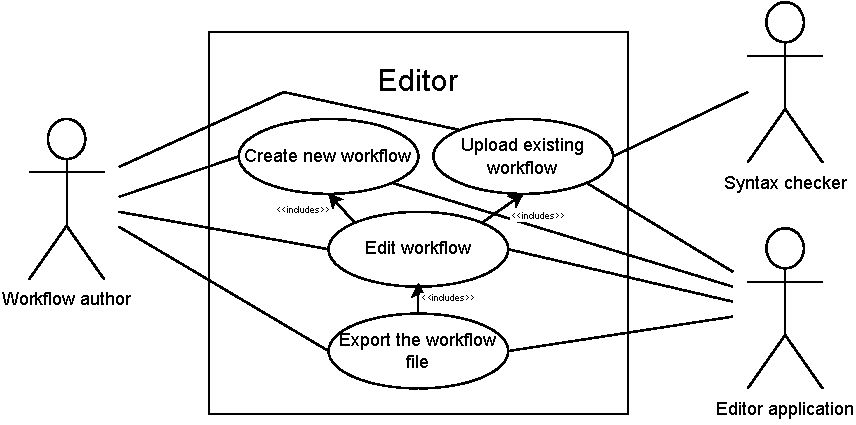
\includegraphics{./img/editorUC.pdf}
    \caption{Editor - Use Case UML diagram}
\end{figure}

% \begin{figure}[h!]
%     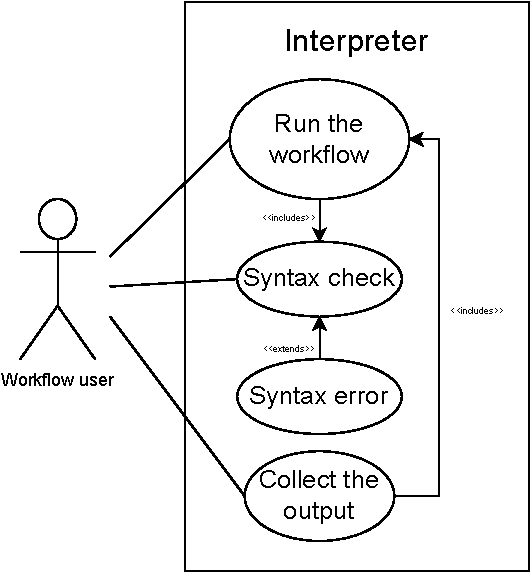
\includegraphics{./img/interpreterUC.pdf}
%     \caption{Interpreter - Use Case UML diagram}
% \end{figure}
